%%____________________________________________________________________________||
\section{Data sets and simulation}
\label{sec:datasets}

\subsection{Primary data sets, certification, and integrated luminosity}

In this analysis, we use proton-proton collision data at $\sqrt{s} =
13\TeV$. The data set collected in 2016 corresponds to an integrated
luminosity of $35.9 \pm 0.9~\ifb$~\cite{lumi}. The studies reported in
this AN are based on control regions populated with the full 2016 data
set.

Table~\ref{tab:cert_json} specifies the JSON file used to identify the
certified data.  Table~\ref{tab:datasets_data} lists the names of the
primary data sets used in this analysis.

\begin{table}[h!]
  \topcaption{The JSON file used to define the certified data set of
    35.9~\ifb} 
  \footnotesize
  %latex.default(d, title = NULL, booktabs = FALSE, width = 3, rowname = NULL,     helvetica = FALSE, caption.loc = "bottom", ...)%
\begin{center}
\begin{tabular}{c}
\hline\hline
\verb!Cert_271036-276811_13TeV_PromptReco_Collisions16_JSON.txt!\tabularnewline
\hline
\end{tabular}\end{center}
 
  \label{tab:cert_json}
\end{table}

\subsection{Blinding statement}

The data in the signal region is currently blinded, with the exception
of 4.5~\ifb of the certified data set, which comprises a sample of
events selected randomly (1 in 8) from throughout the full data taking
period. \fixme{ARE WE DOING THIS?!}

\subsection{Simulated event samples}

Tables~\ref{tab:datasets_bkg} and~\ref{tab:datasets_bkg2} list the
simulated event samples of all relevant standard model background
processes for this analysis.

The dominant SM processes in the signal and control regions, \znunu\ +
jets, W + jets, \ttbar\ + jets, Drell--Yan ($\cPq\bar{\cPq} \to
\PZ/\gamma^* \to \ell^+\ell^-$) + jets, and \gj, are generated at
leading order (LO) using the {\MADGRAPH{}5\_a\MCATNLO} 2.2.2 generator
code~\cite{Alwall2014}. These samples are listed in
Table~\ref{tab:datasets_bkg}.

The {\MADGRAPH{}5\_a\MCATNLO} 2.2.2 code is also used at LO to
generate QCD multijet events, as well as W + jets and Z + jets via
vector boson fusion. The \MADGRAPH{} code is also used to generate at
next-to-leading order (NLO) in the strong coupling constant
($\alpha_\textrm{s}$) samples of s-channel production of single top
and ttW, ttZ, and ttG events. The t-channel and tW-channel single top
samples, as well as ttH samples, are generated using
\POWHEG~\cite{}. The diboson samples (WW, WZ, and ZZ) are generated
using \PYTHIA~\cite{}. These samples are listed in
Table~\ref{tab:datasets_bkg2}.

The {NNPDF}3.0 LO and NLO~\cite{nnpdf} parton distribution functions
(PDFs) are used, respectively, with the LO and NLO generators
described above. The \PYTHIA program with the CUETP8M1 underlying
event tune~\cite{Khachatryan:2015pea} is used to describe parton
showering and hadronisation for all simulated samples, except ttH that
uses CUETP8M2.

The dominant background processes simulated with \MADGRAPH{}@LO
(\znunu\ + jets, Drell--Yan ($\cPq\bar{\cPq} \to \PZ/\gamma^* \to
\ell^+\ell^-$) ($q\bar{q} \ra Z/\gamma \ra l^+l^-$) + jets, \gj, W +
jets, and QCD multijet events) are produced according to the
generator-level scalar sum of partonic transverse energies (``parton
\scalht''). The \ttbar\ + jets samples are also produced according to
the fully or semi-lepton decay of \ttbar\ system. These ``exclusive''
subsamples are filtered according to parton \scalht, in order to
remove any overlaps, and are then ``stitched'' together to provide an
effective inclusive sample that allows for a high effective
intergrated luminosity in the tails of the parton \scalht
distributions.

Inclusive simulated event samples are normalised to inclusive cross
sections calculated with (N)NLO precision. The full detector response
is simulated using the \GEANTfour~\cite{geant} package for these
samples. Each ``exclusive'' subsample is accompanied by an exclusive
LO cross section calculation, which is used to normalise the simulated
event counts to the integrated luminosity. Any \kfactors required to
go from LO to (N)NLO cross sections are typically determined using a
corresponding inclusive sample, which are then applied to each
subsample. The cross sections used for each sample are listed in
Tables~\ref{tab:datasets_bkg} and~\ref{tab:datasets_bkg2}.

The full parton \scalht distribution obtained from the ``stitched''
subsamples relative to that obtained from the corresponding inclusive
sample are shown in Fig.~\ref{fig:Lhe_Ht} (in
Appendix~\ref{app:datasets}), with the bin-by-bin derivative drawn
below. The stitched subsamples demonstate a smooth behaviour
compatible with the inclusive samples.

Table~\ref{tab:datasets_signal} lists the simulated events samples of
signal processes used in this analysis. The event samples for SUSY
signal models involving gluino or squark pair production in
association with up to two additional partons are generated at LO with
{\MADGRAPH{}5\_a\MCATNLO}, and the decay of the SUSY particles is
performed with \PYTHIA 8.205~\cite{pythia}. Inclusive,
process-dependent, signal production cross sections are calculated
with NLO plus next-to-leading-logarithmic (NLL)
accuracy~\cite{Beenakker:1996ch, PhysRevLett.102.111802,
  PhysRevD.80.095004, 1126-6708-2009-12-041,
  doi:10.1142/S0217751X11053560, susynlo}. The theoretical systematic
uncertainties are typically dominated by the parton density function
(PDF) uncertainties, evaluated using the
CTEQ6.6~\cite{Nadolsky:2008zw} and MSTW2008~\cite{Martin:2009iq} PDFs.
The detector response for signal models is provided by the CMS fast
simulation package~\cite{fastsim}.

\subsection{Reducing statistical uncertainties from simulation at high \texorpdfstring{\nb}{Nb}}

In order to maximise sensitivity to potential new physics signatures
in final states with multiple b-quark jets, a method that improves the
statistical power of simulated event samples at high values of \nb is
employed. This method is known as the ``formula method''. The
resulting improvement in the statistical precision of the simulation,
and systematic uncertainties associated with the method, are
propagated through the analysis.

The distribution of the number of bjets (\nb) is estimated from
generator-level information contained in the simulation. The number of
reconstruction-level jets matched to underlying bottom quarks
($\nb^{\rm gen}$), charm quarks ($n_{\rm c}^{\rm gen}$), and
light-flavoured (LF) partons, i.e. $u,d,s$ quarks and gluons ($n_{\rm
  LF}^{\rm gen}$) per event, $N(\nb^{\rm gen},n_{\rm c}^{\rm
  gen},n_{\rm LF}^{\rm gen})$, is recorded in bins of (\njet ,
\scalht, \mht).  The matching between truth-level partons and
reconstruction-level jets is achieved with a matching algorithm
recommended by the BTV POG~\cite{btagMCTools}.  The b-tagging
efficiency, $\epsilon_{\rm b}$, and mistag probabilities,
$\epsilon_{\rm c}$ and $\epsilon_{\rm LF}$, are also determined from
simulation in bins of (\njet, \scalht, \mht), with each efficiency or
mistag probability determined per bin by averaging over jet $p_{\rm
  T}$ and $\eta$. Corrections are applied on a jet-by-jet basis to
each of $\epsilon_{\rm b}$, $\epsilon_{\rm c}$, and $\epsilon_{\rm
  LF}$ in order to match the corresponding measurements from
data. These corrections, or ``scale factors'', are provided by the BTV
POG~\cite{btagMCTools}.

The above information is sufficient to predict the total number of
b-tagged jets in the event $n^{\rm tag} \equiv n_{\rm b}^{\rm tag} +
n_{\rm c}^{\rm tag} + n_{\rm LF}^{\rm tag}$ and thus also determine the
event yield $N(n^{\rm tag})$ from simulation for a given bin in
(\njet,~\scalht,~\mht) with the expression:
\begin{equation}
  \label{equ:btag-formula}
  N(n^{\rm tag}) = \sum_{n_{i}^{\rm gen}} N(n_{\rm b}^{\rm gen},n_{\rm
    c}^{\rm gen},n_{\rm LF}^{\rm gen}) \times (\sum_{n_{i}^{\rm
      tag}}P_{\rm b}\times P_{\rm c} \times P_{\rm LF}) 
\end{equation}
where $n_{\rm b}^{\rm tag}$, $n_{\rm c}^{\rm tag}$ and $n_{\rm
  LF}^{\rm tag}$ are the number of reconstructed and b-tagged jets
which are matched to a b, c, and LF quark respectively and $P_{i} =
P_{\mathrm{binomial}}(n_{i}^{\rm tag}; n_{i}^{\rm gen}, \epsilon_{i})$
is the usual binomial probability density.

As a simple example, consider a bin with 2 reconstructed jets, in
which 1000 events contain 2 light-flavoured jets, i.e. $(n_{\rm
  b}^{\rm gen} = 0,n_{\rm c}^{\rm gen} = 0,n_{\rm LF}^{\rm gen} = 2)$
and 500 events contain 1 light-flavoured jet and 1 b-jet,
i.e. $(n_{\rm b}^{\rm gen} = 1,n_{\rm c}^{\rm gen} = 0,n_{\rm LF}^{\rm
  gen} = 1)$.  In this exercise, we assume a b-tag efficiency
$\epsilon_{\rm b} = 0.65$ and a light-flavour (mistag) efficiency
$\epsilon_{\rm LF} = 0.01$.  The MC yields for the 3 b-tag
multiplicities are then calculated as follows:
\begin{align*}
%% \begin{split}
N(0) = & \; 1000\times (1-\epsilon_{\rm LF})^2 \;+                                \\
       & \; \phantom{1}500\times(1-\epsilon_{\rm b})\times(1-\epsilon_{\rm LF})   \\
     = & \; 1153.35                                                               \\
N(1) = & \; 1000\times (1-\epsilon_{\rm LF})\times \epsilon_{\rm LF} \times 2 \;+ \\
       & \; \phantom{1}500\times (1-\epsilon_{\rm b})\times\epsilon_{\rm LF} \;+\;  
       500\times \epsilon_{\rm b} \times (1-\epsilon_{\rm LF})                    \\
     = & \; \phantom{1}343.3                                                      \\
N(2) = & \; \phantom{1}500\times \epsilon_{\rm b} \times \epsilon_{\rm LF} \;+    \\
       & \; 1000\times \epsilon_{\rm LF}^2                                        \\
     = & \; \phantom{100}3.35                                                     \\
%% \end{split}
\end{align*}
  
The method exploits the ability to make precise measurements of
$N(n_{\rm b}^{\rm gen},n_{\rm c}^{\rm gen},n_{\rm LF}^{\rm gen})$,
$\epsilon$, \fixme{$f_{\rm c}$, and $f_{\rm LF}$} independently of $n_{\rm b}$,
which means that event yields for a given b-quark jet multiplicity can
be predicted with a higher statistical precision than obtained
directly from simulation. Precise measurements of $f_{\rm c}$ and
$f_{\rm LF}$ are particularly important for events with $n_{\rm b} \geq
3$, which often occur in the SM because of the presence of mistagged
jets in the event. In this case, the largest background is \ttbar,
with two correctly tagged b-quark jets and an additional mistagged jet
originating from a charm quark or light-flavoured parton.

\fixme{IMO, WE SHOULD REVERT TO THE USE OF $f_c$ and $f_q$ FOR MISTAG PROBS}

A simulation-based validation (\ie an ``MC closure test'') of the
method is provided in Sec.~\ref{sec:}.

As stated above, the uncertainties in the data/simulation scale factor
corrections applied to the efficiencies and mistag probabilities
determined from simulation are propagated through the analysis. The
resulting systematic uncertainty in the estimation of yields for
events categorised by \nb depends strongly on whether an extrapolation
in \nb is required to estimate a particular background process in the
signal region. These details are covered in Secs.~\ref{sec:}. 

\begin{table}[h!]
  \topcaption{List of primary data sets used in this analysis.}
  \footnotesize 
  \begin{center}
\begin{tabular}{l}
\hline\hline
\multicolumn{1}{c}{Data set}\tabularnewline
\hline
\verb!/HTMHT/Run2016B-23Sep2016-v3/MINIAOD!\tabularnewline
\verb!/HTMHT/Run2016C-23Sep2016-v1/MINIAOD!\tabularnewline
\verb!/HTMHT/Run2016D-23Sep2016-v1/MINIAOD!\tabularnewline
\verb!/HTMHT/Run2016E-23Sep2016-v1/MINIAOD!\tabularnewline
\verb!/HTMHT/Run2016F-23Sep2016-v1/MINIAOD!\tabularnewline
\verb!/HTMHT/Run2016G-23Sep2016-v2/MINIAOD!\tabularnewline
\verb!/HTMHT/Run2016H-PromptReco-v2/MINIAOD!\tabularnewline
\verb!/HTMHT/Run2016H-PromptReco-v3/MINIAOD!\tabularnewline
\verb!/JetHT/Run2016B-23Sep2016-v2/MINIAOD!\tabularnewline
\verb!/JetHT/Run2016C-23Sep2016-v2/MINIAOD!\tabularnewline
\verb!/JetHT/Run2016D-23Sep2016-v2/MINIAOD!\tabularnewline
\verb!/JetHT/Run2016E-23Sep2016-v1/MINIAOD!\tabularnewline
\verb!/JetHT/Run2016F-23Sep2016-v1/MINIAOD!\tabularnewline
\verb!/JetHT/Run2016G-23Sep2016-v2/MINIAOD!\tabularnewline
\verb!/JetHT/Run2016H-PromptReco-v2/MINIAOD!\tabularnewline
\verb!/JetHT/Run2016H-PromptReco-v3/MINIAOD!\tabularnewline
\verb!/MET/Run2016B-23Sep2016-v3/MINIAOD!\tabularnewline
\verb!/MET/Run2016C-23Sep2016-v1/MINIAOD!\tabularnewline
\verb!/MET/Run2016D-23Sep2016-v1/MINIAOD!\tabularnewline
\verb!/MET/Run2016E-23Sep2016-v1/MINIAOD!\tabularnewline
\verb!/MET/Run2016F-23Sep2016-v1/MINIAOD!\tabularnewline
\verb!/MET/Run2016G-23Sep2016-v1/MINIAOD!\tabularnewline
\verb!/MET/Run2016H-PromptReco-v2/MINIAOD!\tabularnewline
\verb!/SingleMuon/Run2016B-23Sep2016-v3/MINIAOD!\tabularnewline
\verb!/SingleMuon/Run2016C-23Sep2016-v1/MINIAOD!\tabularnewline
\verb!/SingleMuon/Run2016D-23Sep2016-v1/MINIAOD!\tabularnewline
\verb!/SingleMuon/Run2016E-23Sep2016-v1/MINIAOD!\tabularnewline
\verb!/SingleMuon/Run2016F-23Sep2016-v1/MINIAOD!\tabularnewline
\verb!/SingleMuon/Run2016G-23Sep2016-v1/MINIAOD!\tabularnewline
\verb!/SingleMuon/Run2016H-PromptReco-v2/MINIAOD!\tabularnewline
\verb!/SingleMuon/Run2016H-PromptReco-v3/MINIAOD!\tabularnewline
\verb!/SinglePhoton/Run2016B-23Sep2016-v3/MINIAOD!\tabularnewline
\verb!/SinglePhoton/Run2016C-23Sep2016-v1/MINIAOD!\tabularnewline
\verb!/SinglePhoton/Run2016D-23Sep2016-v1/MINIAOD!\tabularnewline
\verb!/SinglePhoton/Run2016E-23Sep2016-v1/MINIAOD!\tabularnewline
\verb!/SinglePhoton/Run2016F-23Sep2016-v1/MINIAOD!\tabularnewline
\verb!/SinglePhoton/Run2016G-23Sep2016-v1/MINIAOD!\tabularnewline
\verb!/SinglePhoton/Run2016H-PromptReco-v2/MINIAOD!\tabularnewline
\verb!/SinglePhoton/Run2016H-PromptReco-v3/MINIAOD!\tabularnewline
\verb!/DoubleEG/Run2016B-23Sep2016-v3/MINIAOD!\tabularnewline
\verb!/DoubleEG/Run2016C-23Sep2016-v1/MINIAOD!\tabularnewline
\verb!/DoubleEG/Run2016D-23Sep2016-v1/MINIAOD!\tabularnewline
\verb!/DoubleEG/Run2016E-23Sep2016-v1/MINIAOD!\tabularnewline
\verb!/DoubleEG/Run2016F-23Sep2016-v1/MINIAOD!\tabularnewline
\verb!/DoubleEG/Run2016G-23Sep2016-v1/MINIAOD!\tabularnewline
\verb!/DoubleEG/Run2016H-PromptReco-v2/MINIAOD!\tabularnewline
\verb!/DoubleEG/Run2016H-PromptReco-v3/MINIAOD!\tabularnewline
\hline
\end{tabular}\end{center}

  \label{tab:datasets_data}
\end{table}

\begin{table}[h!]
  \centering
  \topcaption{Simulated event samples of SM background processes used
    by this analysis. Symbols used as shorthand are defined at the
    bottom of the table.}
  \fontsize{7}{8.4}\selectfont
  %latex.default(d, title = NULL, booktabs = FALSE, width = 3, rowname = NULL,     helvetica = FALSE, caption.loc = "bottom", ...)%
\begin{center}
\begin{tabular}{ll}
\hline\hline
\multicolumn{1}{c}{Data set}&\multicolumn{1}{c}{Cross section [pb]}\tabularnewline
\hline
\verb!/ZJetsToNuNu_HT-100To200_13TeV-madgraph/[1]-v1/MINIAODSIM! &$3.448\times 10^{+02}$\tabularnewline
\verb!/ZJetsToNuNu_HT-100To200_13TeV-madgraph/[1]_ext1-v1/MINIAODSIM! &$3.448\times 10^{+02}$\tabularnewline
\verb!/ZJetsToNuNu_HT-200To400_13TeV-madgraph/[1]-v1/MINIAODSIM! &$9.553\times 10^{+01}$\tabularnewline
\verb!/ZJetsToNuNu_HT-200To400_13TeV-madgraph/[1]_ext1-v1/MINIAODSIM! &$9.553\times 10^{+01}$\tabularnewline
\verb!/ZJetsToNuNu_HT-400To600_13TeV-madgraph/[1]-v1/MINIAODSIM! &$1.320\times 10^{+01}$\tabularnewline
\verb!/ZJetsToNuNu_HT-400To600_13TeV-madgraph/[1]_ext1-v1/MINIAODSIM! &$1.320\times 10^{+01}$\tabularnewline
\verb!/ZJetsToNuNu_HT-600To800_13TeV-madgraph/[1]-v1/MINIAODSIM! &$3.221\times 10^{+00}$\tabularnewline
\verb!/ZJetsToNuNu_HT-800To1200_13TeV-madgraph/[1]-v1/MINIAODSIM! &$1.474\times 10^{+00}$\tabularnewline
\verb!/ZJetsToNuNu_HT-1200To2500_13TeV-madgraph/[1]-v1/MINIAODSIM! &$3.586\times 10^{-01}$\tabularnewline
\verb!/ZJetsToNuNu_HT-1200To2500_13TeV-madgraph/[1]_ext1-v1/MINIAODSIM! &$3.586\times 10^{-01}$\tabularnewline
\verb!/ZJetsToNuNu_HT-2500ToInf_13TeV-madgraph/[1]-v1/MINIAODSIM! &$8.203\times 10^{-03}$\tabularnewline
\verb!/WJetsToLNu_HT-100To200_[2]/[1]-v1/MINIAODSIM! &$1.627\times 10^{+03}$\tabularnewline
\verb!/WJetsToLNu_HT-100To200_[2]/[1]_ext1-v1/MINIAODSIM! &$1.627\times 10^{+03}$\tabularnewline
\verb!/WJetsToLNu_HT-100To200_[2]/[1]_ext2-v1/MINIAODSIM! &$1.627\times 10^{+03}$\tabularnewline
\verb!/WJetsToLNu_HT-200To400_[2]/[1]-v1/MINIAODSIM! &$4.352\times 10^{+02}$\tabularnewline
\verb!/WJetsToLNu_HT-200To400_[2]/[1]_ext1-v1/MINIAODSIM! &$4.352\times 10^{+02}$\tabularnewline
\verb!/WJetsToLNu_HT-200To400_[2]/[1]_ext2-v1/MINIAODSIM! &$4.352\times 10^{+02}$\tabularnewline
\verb!/WJetsToLNu_HT-400To600_[2]/[1]-v1/MINIAODSIM! &$5.918\times 10^{+01}$\tabularnewline
\verb!/WJetsToLNu_HT-400To600_[2]/[1]_ext1-v1/MINIAODSIM! &$5.918\times 10^{+01}$\tabularnewline
\verb!/WJetsToLNu_HT-600To800_[2]/[1]-v1/MINIAODSIM! &$1.458\times 10^{+01}$\tabularnewline
\verb!/WJetsToLNu_HT-600To800_[2]/[1]_ext1-v1/MINIAODSIM! &$1.458\times 10^{+01}$\tabularnewline
\verb!/WJetsToLNu_HT-800To1200_[2]/[1]-v1/MINIAODSIM! &$6.656\times 10^{+00}$\tabularnewline
\verb!/WJetsToLNu_HT-800To1200_[2]/[1]_ext1-v1/MINIAODSIM! &$6.656\times 10^{+00}$\tabularnewline
\verb!/WJetsToLNu_HT-1200To2500_[2]/[1]-v1/MINIAODSIM! &$1.608\times 10^{+00}$\tabularnewline
\verb!/WJetsToLNu_HT-1200To2500_[2]/[1]_ext1-v1/MINIAODSIM! &$1.608\times 10^{+00}$\tabularnewline
\verb!/WJetsToLNu_HT-2500ToInf_[2]/[1]-v1/MINIAODSIM! &$3.891\times 10^{-02}$\tabularnewline
\verb!/WJetsToLNu_HT-2500ToInf_[2]/[1]_ext1-v1/MINIAODSIM! &$3.891\times 10^{-02}$\tabularnewline
\verb!/TTJets_DiLept_[2]/[1]-v1/MINIAODSIM! &$8.829\times 10^{+01}$\tabularnewline
\verb!/TTJets_DiLept_[2]/[1]_ext1-v1/MINIAODSIM! &$8.829\times 10^{+01}$\tabularnewline
\verb!/TTJets_HT-600to800_[2]/[1]_ext1-v1/MINIAODSIM! &$2.734\times 10^{+00}$\tabularnewline
\verb!/TTJets_HT-800to1200_[2]/[1]_ext1-v1/MINIAODSIM! &$1.121\times 10^{+00}$\tabularnewline
\verb!/TTJets_HT-1200to2500_[2]/[1]_ext1-v1/MINIAODSIM! &$1.979\times 10^{-01}$\tabularnewline
\verb!/TTJets_HT-2500toInf_[2]/[1]_ext1-v1/MINIAODSIM! &$2.368\times 10^{-03}$\tabularnewline
\verb!/TTJets_SingleLeptFromT_[2]/[1]-v1/MINIAODSIM! &$1.827\times 10^{+02}$\tabularnewline
\verb!/TTJets_SingleLeptFromT_[2]/[1]_ext1-v1/MINIAODSIM! &$1.827\times 10^{+02}$\tabularnewline
\verb!/TTJets_SingleLeptFromTbar_[2]/[1]-v1/MINIAODSIM! &$1.827\times 10^{+02}$\tabularnewline
\verb!/TTJets_SingleLeptFromTbar_[2]/[1]_ext1-v1/MINIAODSIM! &$1.827\times 10^{+02}$\tabularnewline
\verb!/DYJetsToLL_M-50_HT-100to200_[2]/[1]-v1/MINIAODSIM! &$1.813\times 10^{+02}$\tabularnewline
\verb!/DYJetsToLL_M-50_HT-100to200_[2]/[1]_ext1-v1/MINIAODSIM! &$1.813\times 10^{+02}$\tabularnewline
\verb!/DYJetsToLL_M-50_HT-200to400_[2]/[1]-v1/MINIAODSIM! &$5.042\times 10^{+01}$\tabularnewline
\verb!/DYJetsToLL_M-50_HT-200to400_[2]/[1]_ext1-v1/MINIAODSIM! &$5.042\times 10^{+01}$\tabularnewline
\verb!/DYJetsToLL_M-50_HT-400to600_[2]/[1]-v1/MINIAODSIM! &$6.984\times 10^{+00}$\tabularnewline
\verb!/DYJetsToLL_M-50_HT-400to600_[2]/[1]_ext1-v1/MINIAODSIM! &$6.984\times 10^{+00}$\tabularnewline
\verb!/DYJetsToLL_M-50_HT-600to800_[2]/[1]-v2/MINIAODSIM! &$1.681\times 10^{+00}$\tabularnewline
\verb!/DYJetsToLL_M-50_HT-800to1200_[2]/[1]-v1/MINIAODSIM! &$7.754\times 10^{-01}$\tabularnewline
\verb!/DYJetsToLL_M-50_HT-1200to2500_[2]/[1]-v1/MINIAODSIM! &$1.862\times 10^{-01}$\tabularnewline
\verb!/DYJetsToLL_M-50_HT-2500toInf_[2]/[1]-v1/MINIAODSIM! &$4.385\times 10^{-03}$\tabularnewline
\verb!/GJets_HT-40To100_[2]/[1]-v1/MINIAODSIM! &$2.079\times 10^{+04}$\tabularnewline
\verb!/GJets_HT-40To100_[2]/[1]_ext1-v1/MINIAODSIM! &$2.079\times 10^{+04}$\tabularnewline
\verb!/GJets_HT-100To200_[2]/[1]-v1/MINIAODSIM! &$9.238\times 10^{+03}$\tabularnewline
\verb!/GJets_HT-100To200_[2]/[1]_ext1-v1/MINIAODSIM! &$9.238\times 10^{+03}$\tabularnewline
\verb!/GJets_HT-200To400_[2]/[1]-v1/MINIAODSIM! &$2.305\times 10^{+03}$\tabularnewline
\verb!/GJets_HT-200To400_[2]/[1]_ext1-v1/MINIAODSIM! &$2.305\times 10^{+03}$\tabularnewline
\verb!/GJets_HT-400To600_[2]/[1]-v1/MINIAODSIM! &$2.744\times 10^{+02}$\tabularnewline
\verb!/GJets_HT-400To600_[2]/[1]_ext1-v2/MINIAODSIM! &$2.744\times 10^{+02}$\tabularnewline
\verb!/GJets_HT-600ToInf_[2]/[1]-v1/MINIAODSIM! &$9.346\times 10^{+01}$\tabularnewline
\verb!/GJets_HT-600ToInf_[2]/[1]_ext1-v1/MINIAODSIM! &$9.346\times 10^{+01}$\tabularnewline
\hline
\multicolumn{1}{l}{String} & \multicolumn{1}{l}{Symbol} \tabularnewline
\verb!RunIISummer16MiniAODv2-PUMoriond17_80X_mcRun2_asymptotic_2016_TrancheIV_v6! & \verb![1]! \tabularnewline
\verb!TuneCUETP8M1_13TeV-madgraphMLM-pythia8! & \verb![2]! \tabularnewline
\hline
\hline
\end{tabular}\end{center}

  \label{tab:datasets_bkg}
\end{table}

\begin{table}[h!]
  \centering
  \topcaption{Simulated event samples of SM background processes used
    by this analysis. Symbols used as shorthand are defined at the
    bottom of the table.}
  \fontsize{7}{8.4}\selectfont
  %latex.default(d, title = NULL, booktabs = FALSE, width = 3, rowname = NULL,     helvetica = FALSE, caption.loc = "bottom", ...)%
\begin{center}
\begin{tabular}{ll}
\hline\hline
\multicolumn{1}{c}{Data set}&\multicolumn{1}{c}{Cross section [pb]}\tabularnewline
\hline
\verb!/QCD_HT100to200_[2]/[1]-v1/MINIAODSIM! &$2.799\times 10^{+07}$\tabularnewline
\verb!/QCD_HT200to300_[2]/[1]-v1/MINIAODSIM! &$1.712\times 10^{+06}$\tabularnewline
\verb!/QCD_HT200to300_[2]/[1]_ext1-v1/MINIAODSIM! &$1.712\times 10^{+06}$\tabularnewline
\verb!/QCD_HT300to500_[2]/[1]-v1/MINIAODSIM! &$3.477\times 10^{+05}$\tabularnewline
\verb!/QCD_HT300to500_[2]/[1]_ext1-v1/MINIAODSIM! &$3.477\times 10^{+05}$\tabularnewline
\verb!/QCD_HT500to700_[2]/[1]-v1/MINIAODSIM! &$3.210\times 10^{+04}$\tabularnewline
\verb!/QCD_HT500to700_[2]/[1]_ext1-v2/MINIAODSIM! &$3.210\times 10^{+04}$\tabularnewline
\verb!/QCD_HT700to1000_[2]/[1]-v1/MINIAODSIM! &$6.831\times 10^{+03}$\tabularnewline
\verb!/QCD_HT700to1000_[2]/[1]_ext1-v1/MINIAODSIM! &$6.831\times 10^{+03}$\tabularnewline
\verb!/QCD_HT1000to1500_[2]/[1]-v1/MINIAODSIM! &$1.207\times 10^{+03}$\tabularnewline
\verb!/QCD_HT1000to1500_[2]/[1]_ext1-v1/MINIAODSIM! &$1.207\times 10^{+03}$\tabularnewline
\verb!/QCD_HT1500to2000_[2]/[1]-v1/MINIAODSIM! &$1.199\times 10^{+02}$\tabularnewline
\verb!/QCD_HT1500to2000_[2]/[1]_ext1-v1/MINIAODSIM! &$1.199\times 10^{+02}$\tabularnewline
\verb!/QCD_HT2000toInf_[2]/[1]-v1/MINIAODSIM! &$2.524\times 10^{+01}$\tabularnewline
\verb!/QCD_HT2000toInf_[2]/[1]_ext1-v1/MINIAODSIM! &$2.524\times 10^{+01}$\tabularnewline
\verb!/ST_s-channel_4f_leptonDecays_[3]/[1]-v1/MINIAODSIM! &$3.344\times 10^{+00}$\tabularnewline
\verb!/ST_tW_antitop_5f_inclusiveDecays_[4]/[1]_ext1-v1/MINIAODSIM! &$3.560\times 10^{+01}$\tabularnewline
\verb!/ST_tW_top_5f_inclusiveDecays_[4]/[1]_ext1-v1/MINIAODSIM! &$3.560\times 10^{+01}$\tabularnewline
\verb!/ST_t-channel_antitop_4f_inclusiveDecays_[5]/[1]-v1/MINIAODSIM! &$8.095\times 10^{+01}$\tabularnewline
\verb!/ST_t-channel_top_4f_inclusiveDecays_[5]/[1]-v1/MINIAODSIM! &$1.360\times 10^{+02}$\tabularnewline
\verb!/TTWJetsToLNu_[6]FXFX-madspin-pythia8/[1]_ext1-v3/MINIAODSIM! &$2.043\times 10^{-01}$\tabularnewline
\verb!/TTWJetsToLNu_[6]FXFX-madspin-pythia8/[1]_ext2-v1/MINIAODSIM! &$2.043\times 10^{-01}$\tabularnewline
\verb!/TTWJetsToQQ_[6]FXFX-madspin-pythia8/[1]-v1/MINIAODSIM! &$4.062\times 10^{-01}$\tabularnewline
\verb!/TTZToLLNuNu_M-10_[6]-pythia8/[1]_ext1-v1/MINIAODSIM! &$2.529\times 10^{-01}$\tabularnewline
\verb!/TTZToQQ_[6]-pythia8/[1]-v1/MINIAODSIM! &$5.297\times 10^{-01}$\tabularnewline
\verb!/TTGJets_[6]FXFX-madspin-pythia8/[1]-v1/MINIAODSIM! &$3.697\times 10^{+00}$\tabularnewline
\verb!/TTGJets_[6]FXFX-madspin-pythia8/[1]_ext1-v1/MINIAODSIM! &$3.697\times 10^{+00}$\tabularnewline
\verb!/ttHToNonbb_M125_TuneCUETP8M2_ttHtranche3_[7]/[1]-v1/MINIAODSIM! &$2.151\times 10^{-01}$\tabularnewline
\verb!/ttHTobb_M125_TuneCUETP8M2_ttHtranche3_[7]/[1]-v1/MINIAODSIM! &$2.934\times 10^{-01}$\tabularnewline
\verb!/WW_TuneCUETP8M1_13TeV-pythia8/[1]-v1/MINIAODSIM! &$1.139\times 10^{+02}$\tabularnewline
\verb!/WW_TuneCUETP8M1_13TeV-pythia8/[1]_ext1-v1/MINIAODSIM! &$1.139\times 10^{+02}$\tabularnewline
\verb!/WZ_TuneCUETP8M1_13TeV-pythia8/[1]-v1/MINIAODSIM! &$4.713\times 10^{+01}$\tabularnewline
\verb!/WZ_TuneCUETP8M1_13TeV-pythia8/[1]_ext1-v1/MINIAODSIM! &$4.713\times 10^{+01}$\tabularnewline
\verb!/ZZ_TuneCUETP8M1_13TeV-pythia8/[1]-v1/MINIAODSIM! &$1.652\times 10^{+01}$\tabularnewline
\verb!/ZZ_TuneCUETP8M1_13TeV-pythia8/[1]_ext1-v1/MINIAODSIM! &$1.652\times 10^{+01}$\tabularnewline
\verb!/EWKWMinus2Jets_WToLNu_M-50_13TeV-madgraph-pythia8/[1]-v1/MINIAODSIM! &$1.000\times 10^{+00}$\tabularnewline
\verb!/EWKWPlus2Jets_WToLNu_M-50_13TeV-madgraph-pythia8/[1]-v1/MINIAODSIM! &$1.000\times 10^{+00}$\tabularnewline
\verb!/EWKZ2Jets_ZToLL_M-50_13TeV-madgraph-pythia8/[1]-v1/MINIAODSIM! &$1.000\times 10^{+00}$\tabularnewline
\verb!/EWKZ2Jets_ZToNuNu_13TeV-madgraph-pythia8/[1]-v1/MINIAODSIM! &$1.000\times 10^{+00}$\tabularnewline
\hline
\multicolumn{1}{l}{String} & \multicolumn{1}{l}{Symbol} \tabularnewline
\verb!RunIISummer16MiniAODv2-PUMoriond17_80X_mcRun2_asymptotic_2016_TrancheIV_v6! & \verb![1]! \tabularnewline
\verb!TuneCUETP8M1_13TeV-madgraphMLM-pythia8! & \verb![2]! \tabularnewline
\verb!13TeV-amcatnlo-pythia8_TuneCUETP8M1! & \verb![3]! \tabularnewline
\verb!13TeV-powheg-pythia8_TuneCUETP8M1! & \verb![4]! \tabularnewline
\verb!13TeV-powhegV2-madspin-pythia8_TuneCUETP8M1! & \verb![5]! \tabularnewline
\verb!TuneCUETP8M1_13TeV-amcatnlo! & \verb![6]! \tabularnewline
\verb!TuneCUETP8M2_ttHtranche3_13TeV-powheg-pythia8! & \verb![7]! \tabularnewline
\hline
\hline
\end{tabular}\end{center}

%\verb!/GJets_DR-0p4_HT-40To100_[2]/[2]-v1/MINIAODSIM! &$1.856\times 10^{+04}$\tabularnewline
%\verb!/GJets_DR-0p4_HT-100To200_[2]/[2]-v1/MINIAODSIM! &$5.000\times 10^{+03}$\tabularnewline
%\verb!/GJets_DR-0p4_HT-200To400_[2]/[2]-v1/MINIAODSIM! &$1.079\times 10^{+03}$\tabularnewline
%\verb!/GJets_DR-0p4_HT-400To600_[2]/[2]-v1/MINIAODSIM! &$1.259\times 10^{+02}$\tabularnewline
%\verb!/GJets_DR-0p4_HT-600ToInf_[2]/[2]-v1/MINIAODSIM! &$4.336\times 10^{+01}$\tabularnewline
%RunIISummer16MiniAODv2-PUMoriond17_qcut19_80X_mcRun2_asymptotic_2016_TrancheIV_v6 [1]

  \label{tab:datasets_bkg2}
\end{table}

\begin{table}[h!]
  \centering
  \topcaption{Simulated event samples of signal processes used
    by this analysis. Symbols used as shorthand are defined at the
    bottom of the table. 
  }
  \footnotesize
  \begin{longtable}{| c | c | c | c | c | c | c | c | c  | }
\caption{Summary of yields of each SM process} \label{tab:table} \\    \hline 
$n_{j}$~$n_{b}$~$H_{T}$ & $t\bar{t}$ & $W+jets$ & $Z \rightarrow \nu\nu$ & $DY+jets$ & $Single Top$ & $DiBoson$ & $Multijet$ & Total Yield\\ \hline 
eq2j eq0b 200 & 103.49 & 1026.57 & 1148.86 & 18.24 & 15.98 & 72.15 & 0.00 & 2385.28\\ \hline 
eq2j eq0b 250 & 74.63 & 1050.96 & 1312.16 & 16.09 & 15.33 & 74.25 & 10.11 & 2553.53\\ \hline 
eq2j eq0b 300 & 32.27 & 664.60 & 941.01 & 9.13 & 6.52 & 42.69 & 2.85 & 1699.07\\ \hline 
eq2j eq0b 350 & 12.65 & 395.06 & 569.00 & 5.50 & 1.62 & 17.06 & 1.33 & 1002.24\\ \hline 
eq2j eq0b 400 & 7.22 & 316.98 & 551.29 & 3.96 & 2.22 & 14.28 & 1.51 & 897.46\\ \hline 
eq2j eq0b 500 & 1.33 & 102.97 & 190.11 & 0.79 & 0.01 & 2.12 & 0.00 & 297.31\\ \hline 
eq2j eq0b 600 & 0.47 & 50.93 & 111.12 & 0.29 & 0.54 & 2.69 & 0.00 & 166.04\\ \hline 
eq2j eq0b 800 & 0.52 & 86.65 & 146.22 & 0.39 & 0.00 & 3.16 & 0.00 & 236.94\\ \hline 
eq3j eq1b 200 & 0.57 & 0.00 & 0.32 & 0.00 & 0.00 & 0.00 & 0.00 & 0.89\\ \hline 
eq3j eq1b 250 & 64.13 & 17.16 & 27.10 & 0.54 & 5.36 & 1.22 & 0.00 & 115.51\\ \hline 
eq3j eq1b 300 & 122.13 & 56.55 & 74.29 & 1.00 & 13.99 & 2.69 & 0.00 & 270.64\\ \hline 
eq3j eq1b 350 & 94.34 & 52.60 & 82.06 & 0.85 & 13.66 & 5.30 & 6.22 & 255.03\\ \hline 
eq3j eq1b 400 & 71.61 & 66.57 & 99.75 & 0.82 & 15.02 & 3.06 & 0.43 & 257.26\\ \hline 
eq3j eq1b 500 & 11.23 & 18.94 & 42.91 & 0.24 & 1.88 & 1.61 & 0.00 & 76.82\\ \hline 
eq3j eq1b 600 & 2.92 & 10.44 & 26.73 & 0.12 & 0.66 & 1.20 & 0.00 & 42.06\\ \hline 
eq3j eq1b 800 & 1.93 & 11.73 & 29.27 & 0.07 & 0.54 & 1.37 & 0.00 & 44.92\\ \hline 
eq4j eq2b 200 & 0.00 & 0.00 & 0.00 & 0.00 & 0.00 & 0.00 & 0.00 & 0.00\\ \hline 
eq4j eq2b 250 & 0.20 & 0.00 & 0.02 & 0.00 & 0.00 & 0.00 & 0.00 & 0.22\\ \hline 
eq4j eq2b 300 & 18.30 & 0.75 & 1.98 & 0.01 & 1.38 & 0.00 & 0.00 & 22.42\\ \hline 
eq4j eq2b 350 & 56.98 & 4.03 & 6.78 & 0.08 & 3.56 & 0.00 & 0.00 & 71.43\\ \hline 
eq4j eq2b 400 & 86.02 & 6.97 & 12.42 & 0.11 & 4.54 & 0.60 & 0.00 & 110.66\\ \hline 
eq4j eq2b 500 & 21.45 & 2.68 & 7.27 & 0.05 & 2.76 & 0.25 & 0.00 & 34.46\\ \hline 
eq4j eq2b 600 & 5.24 & 2.02 & 4.38 & 0.02 & 1.26 & 0.05 & 0.00 & 12.98\\ \hline 
eq4j eq2b 800 & 2.66 & 0.00 & 3.79 & 0.02 & 0.58 & 0.00 & 0.00 & 7.06\\ \hline 
ge5j eq0b 200 & 0.00 & 0.00 & 0.00 & 0.00 & 0.00 & 0.00 & 0.00 & 0.00\\ \hline 
ge5j eq0b 250 & 0.00 & 0.00 & 0.00 & 0.00 & 0.00 & 0.00 & 0.00 & 0.00\\ \hline 
ge5j eq0b 300 & 0.03 & 0.00 & 0.05 & 0.00 & 0.00 & 0.00 & 0.00 & 0.07\\ \hline 
ge5j eq0b 350 & 6.96 & 8.88 & 7.98 & 0.26 & 0.00 & 0.39 & 0.02 & 24.49\\ \hline 
ge5j eq0b 400 & 57.77 & 102.86 & 111.49 & 1.65 & 3.35 & 4.48 & 0.00 & 281.60\\ \hline 
ge5j eq0b 500 & 41.04 & 96.56 & 124.97 & 1.30 & 1.62 & 1.67 & 8.83 & 275.99\\ \hline 
ge5j eq0b 600 & 26.59 & 91.74 & 128.08 & 0.96 & 2.62 & 3.95 & 1.72 & 255.67\\ \hline 
ge5j eq0b 800 & 16.75 & 67.00 & 130.94 & 0.76 & 1.84 & 2.45 & 6.82 & 226.57\\ \hline 
    \hline 
    \hline 
\end{longtable}

  \label{tab:datasets_signal}
\end{table}

\clearpage
\subsection{Corrections to simulation for SM processes}
\label{sec:sim-corrs}

\subsubsection{Pileup}
\label{sec:pileup-reweighting}

To model the effects of multiple pp collisions within the same or
neighbouring bunch crossings (pileup), all simulated events are
generated with a nominal distribution of pp interactions per bunch
crossing. On average, approximately twenty different pp collisions,
identifiable via their primary interaction vertex, are reconstructed
per event. The simulated event samples are reweighted to match the
pileup distribution as measured in data. This procedure is called
\textit{pileup reweighting}.

In deriving the pileup reweighting factors, we follow the
recommendation by the physics validation group
\cite{twiki-PdmVPileUpDescription, twiki-PileupJSONFileforData}. In
the recommendation, the reweighting factors are a function of the
variable called \verb!nTrueInt!.

The variable \verb!nTrueInt! is the parameter of the Poisson
distribution from which the numbers of pileup interactions are drown
as random numbers. In each simulated event, the number of the in-time
pileup interactions and the number of the interactions in each
neighbouring bunch crossing to simulate the out-of-time pileup are
random numbers from the Poisson distribution with the same parameter,
\verb!nTrueInt!. The value of \verb!nTrueInt! is not a constant of the
data set. It is a random number from the distribution specified in
Ref. \cite{github-mix_2016_25ns_SpringMC_PUScenarioV1_PoissonOOTPU_cfi}.

The \verb!nTrueInt! in the data is the average pileup interactions for
a colliding bunch pair in a lumi section. The distribution of
\verb!nTrueInt! in the data is derived from the measured instantaneous
luminosity for each colliding bunch pair in each lumi section and the
cross section of the total inelastic pp interaction. We use the method
in Ref. \cite{twiki-PileupJSONFileforData} in deriving the
distribution with the recommended value of 63.00~mb as the minimum
bias cross section. In addition, we derive distributions with $\pm
5\%$ of the variations of the minimum bias cross section, i.e,
66.15~mb and 59.850~mb.

The pileup reweighting factors are the ratios of the distributions of
\verb!nTrueInt! in the data and in the simulated events and are
normalised so as to preserve the number of the simulated events.

\begin{figure}[h!]
  \centering
  \subfigure[]{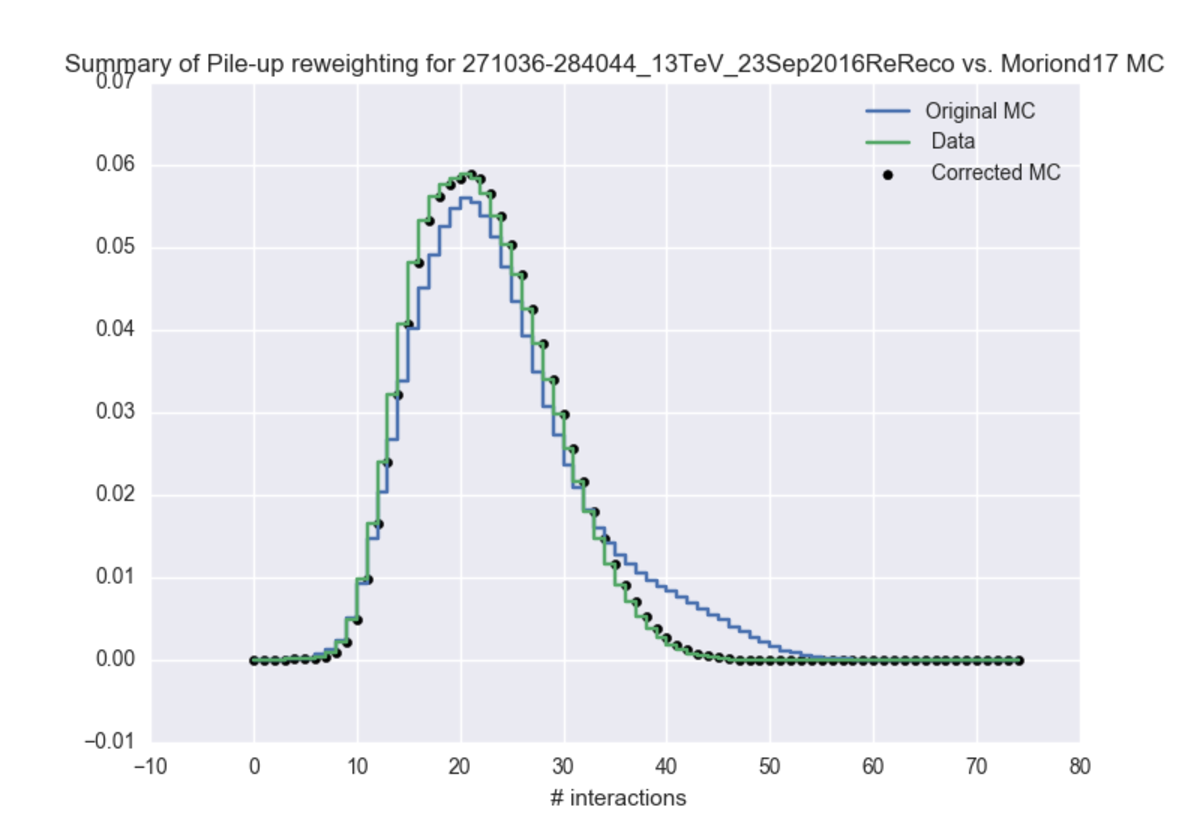
\includegraphics[width=0.5\textwidth]{figures/pileup_reweighting/summarized_data.pdf}} ~
  \subfigure[]{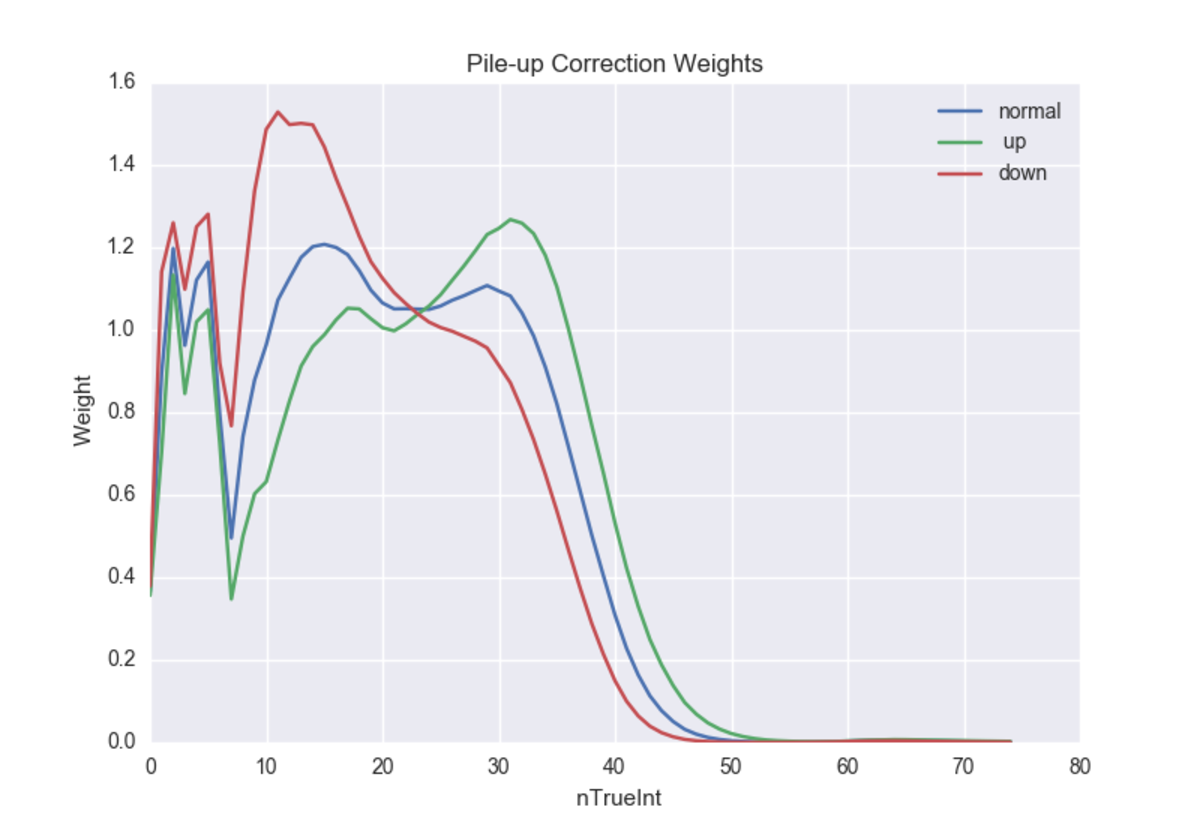
\includegraphics[width=0.5\textwidth]{figures/pileup_reweighting/tbl_20170125_01-tbl_corr_nTrueInt.pdf}} 
  \caption{(a) The distribution of the average numbers of the
    inelastic interactions per colliding bunch pair per lumi section
    in the data, corresponding distribution in the simulated events,
    and that of the reweighted simulated events. (b) The weights
    applied to simulated events as a function of the average number of
    the inelastic interactions per colliding bunch pair per lumi
    section.}
  \label{f044_corr_nTrueInt_data_mc_norm}
\end{figure}

Figure~\ref{f044_corr_nTrueInt_data_mc_norm} shows the distributions
of \verb!nTrueInt! in the data, simulated events and reweighted
simulated events. The figure demonstrates that the reweighted
simulated events have the distribution of \verb!nTrueInt! nearly
identical to that in the data. 
We note that the simulation does not contain events with 37 or more
overlapping pp interactions, while the data do, causing the MC
weighted distribution not to match perfectly the data. This small
issue will be recovered once the new MC samples with updated PU
profile will be available.

\subsubsection{Lepton and photon scale factors}

Simulation mismodelling of efficiencies related to object
identification and isolation requirements are mitigated by the use of
scale factors. Corrections related to trigger and tracking
reconstruction efficiencies are also considered. Typically, the scale
factors are near-unity and are determined by the POGs or the SUSY
lepton scale factor working group. We follow the SUSY Moriond17
recommendations, detailed here~\cite{susymoriond}. Further details
are given in later sections. 

\subsubsection{Jet energy scale corrections and b-tag scale factors}
\label{sec:jecs-and-btag-sf}

Jet energy scale corrections and b-tag scale factors are applied to
the simulated event samples following the JetMET and BTV POG
recommendations. Details in subsequent sections. 

\subsubsection{Boson-\texorpdfstring{\Pt}{pT}-dependent NLO corrections}

The \MADGRAPH generator is used to simulate W + jets, DY + jets,
\znunu\ + jets, and \gj at leading order. Missing higher order
corrections, which can result in a modified boson \Pt distribution,
can be determined from (QCD) NLO simulation and (EWK) theory
calculations, as done by the the monojet search in the EXO
PAG~\cite{}. We do not apply these corrections to our simulated
samples, but instead include the corrections as a source of systematic
uncertainty in our transfer factors via a nuisance in our likelihood
model. Further details are given in Sec.~\ref{sec:}.

\subsubsection{\texorpdfstring{\nisr}{Nisr} reweighting for \texorpdfstring{\ttbar}{TTbar}}

To improve on the \MADGRAPH modelling of the multiplicity of
additional jets from initial state radiation (ISR), the SUSY group
recommends to reweight \MADGRAPH \ttbar Monte Carlo events according
to the number of ISR jets ($N_J^{ISR}$) identified in the event so as
to improve the jet multiplicity agreement with data. The reweighting
factors vary between 0.92 and 0.51 for $N_J^{ISR}$ between 1 and 6. In
this analysis, we categorise identically the events in the control and
signal regions according to the number of jets reconstructed in an
event. Hence such a correction is expected to have very little impact
on the final result. 

Further, this procedure attempts to correct for the mismodelling of
associated jet production for \ttbar processes, which may be due to
missing higher-order calculations in the LO \MADGRAPH MC. Hence, for
consistency with the V + jets samples (also produced with
\MADGRAPH{}@LO), we prefer not to apply the $N_J^{ISR}$ corrections to
our simulated samples, but instead include the corrections as a source
of systematic uncertainty in our transfer factors via a nuisance in
our likelihood model. Further details are given in Sec.~\ref{sec:}.
\fixme{ARE WE DOING THIS? ``We take one half of the deviation from
  unity as the systematic uncertainty on these reweighting factors.''}

\subsection{Corrections to simulation for signal processes}

\fixme{IDENTIFY THE MAIN CORRECTIONS TO BE APPLIED, AS DETAILED IN THE
SUSY TWIKI}

%%____________________________________________________________________________||
